%
% CHAPTER Versuch 4
%
\chapter{Pixelfehler}
Je nach Qualität des Bildsensors gibt es durch den Fertigungsprozess funktionsuntüchtige Pixel, welche das Bild verfälschen, diese gilt es in diesem Kapitel zu korrigieren.
\label{chap:Pixelfehler}

\section{Fragestellung, Messprinzip, Aufbau, Messmittel}
Um unser Testbild \ref{img:Grauwertkeil} zu korrigieren, gilt es nun den durch das Dunkelbild berechnete Offset der Pixel zu entfernen. Desweiteren wird das Bild noch durch das in V3 \ref{chap:VERSUCH_3} berechnete und normierte Weissbild geteilt um die Sensitivität anzupassen.
Im Anschluss wird uns ein Pythonskript TODO REF die differenz der einzelnen Bereiche zwischen dem Original Graukeilbild und dem korrigierten Graukeilbild berechnen. Hierzu wird das Bild zunächst in die einzelnen Graustufen zerlegt und im anschluss der durchschnittliche Farbwert dieser Graustufe wie auch die Standartabweichung, was dem rauschen der Pixel entspricht, berechnet. Durch vergleichen dieser Werte sollte sich eine Besserung des Bildes feststellen lassen. Die besserung sollte vorallem im beseitigen des rauschens liegen, was die Standartabweichung der einzelnen Keile sichtbar senken sollte.
\label{chap:VERSUCH_4_FRAGESTELLUNG}

\section{Messwerte}
\begin{figure}[H]
\centering
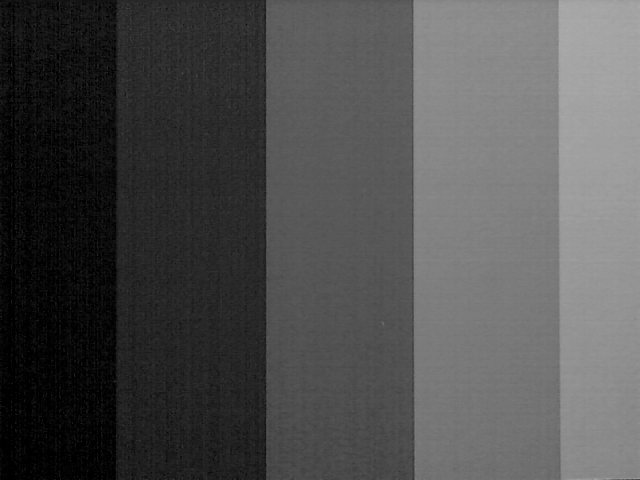
\includegraphics[width=150mm]{graustufen.png}
\caption{Markierter Offset}
\label{img:struckpixel.png}
\end{figure}
\label{chap:VERSUCH_4_MESSWERTE}

\section{Auswertung}
Bei genauerer Betrachtung des Kontrast maximierten Dunkelbildes \ref{img:struckpixel.png} fallen einige weisse Punkte ins Auge. Hierbei handelt es sich um hotpixel, welche durch längere Belichtungszeit in die Sättigung gehen oder um stuckpixel, welche sich stehts auf ihrem maximalwert bleiben $(rot markiert)$
\label{chap:VERSUCH_4_AUSWERTUNG}

\section{Interpretation}
\label{chap:VERSUCH_4_INTERPRETATION}